\label{sec:modeling}
%Basically, an embedded system is given by an application mapped to a platform. The application is a parallel composition of tasks.
The platform we consider consists of a set of cores (processing elements), one shared cache level and a shared DRAM. %and mechanisms to share and control the access to the platform resources like processor schedulers and DRAM connectors. 
The application is given by a set of tasks mapped to different cores. Mainly, application tasks are characterized by their computation times WCET (measured when each task runs in isolation), and the worst case resource access numbers (WCRA) \cite{Nowotsch14} to DRAM and shared cache L2 for both read and write actions. Access requests to shared memory are non-deterministically spread out along the task execution. The reason behind that is that tasks execution, and thereby the issue time of data requests, may vary from one period to another following the changes in the computation environment. 

We use ${\cal T}$ for the set of tasks and ${\cal C}$ for the set of cores. The assumptions about the systems we consider are the following: 
%
\begin{itemize}
\item Tasks are periodic and non-preemptible during CPU use. 
\item Tasks assigned to the same core are arbitrated using a local scheduler. 
\item We consider a local cache (L1) for each core, only one shared cache (L2) and one DRAM for all cores.
%\item We abstract each local cache using a number stating the time for fetching data from it. %The number of local cache misses corresponds to the WCRA number to L2.  
%\item Tasks are assigned statically to PE so that a task always executes on the same core. Later on, but our framework can easily be extended with dynamic assignment to incorporate migration and workload balance.
\end{itemize}

\subsection{Application Model}
An application $AP=\{T_1,..,T_n\}$ is a set of tasks each of which describes the execution model of an individual process. The process behavior is abstracted at task level using WCET and WCRA for both shared cache and DRAM. WCET is the pure execution time, calculated in isolation when a task runs alone on a single core. Regarding data fetching, we consider 2 attributes $\emph{WCRA}_c$ and $\emph{WCRA}_m$ where: $\emph{WCRA}_c$ corresponds to the maximum number of successful accesses (hits) to the shared cache L2; $\emph{WCRA}_m$ is the number of DRAM accesses (corresponds to L2 miss) performed by a given process. Moreover, in order to distinguish between read and write accesses to each shared memory, we denote each of the attributes with $r$ for read and $w$ for write, i.e. $\CR, \CW, \MR$ and $\MW$. This is because read requests make the core stalling (strong impact on isWCET) while write requests do not as they can be performed using dedicated buffers. Such patterns are identifiable using abstract interpretation \cite{Wang2010} and program/cache analysis \cite{Ferdinand1999}, e.g. the PAG tool \cite{PAG}, on a given platform architecture. %As stated earlier, the duration for fetching data from a shared memory varies because of the interference.    

An access request to a shared memory is given by a $\emph{pattern}\in \{L2, DRAM\}$ stating to which memory the access hits and an attribute $RW$ indicates whether it is a read ($r$) or write ($w$) action. Moreover, as we need to keep track of when the requests are issued, so that FR-FCFS algorithm determines the priorities of requests targeting DRAM, we use \emph{issueTime}. 
In fact, \emph{issueTime} is initially empty and will be initialized by a core when the access request is triggered. Accordingly, an access request is formally given by $\emph{req}=\langle \emph{pattern}, RW, \emph{issueTime}\rangle$. 
$\CR$ and $\CW$, respectively $\MR$ and $\MW$, of a given task are then the numbers of read and write accesses to L2, respectively DRAM.

\begin{definition}[Task structure] A task $T$ is given by $\small{\langle \emph{Prd}, \emph{Offset}, \emph{WCET}, \CR, \CW, \MR,\MW, \emph{Dln}, \emph{Pri}\rangle}$ where $\emph{Prd}$ is the task period, $\emph{Offset}$ is the periodic offset, $\emph{WCET}$ is the pure execution time, $\emph{Dln}$ is the relative deadline whereas $\emph{Pri}$ is the priority level associated to $T$.
$\CR, \CW, \MR$ and $\MW$ are described above.
%, whereas $c\_Id$ is the core Id to which the task is allocated. 
\end{definition}

%In order to make the application specification flexible, we do not (statically) specify the identifier of the core to which the task is assigned. The mapping will rather be given during system instantiation i.e. once the target platform is given. 
The behavior of a task is a basically a state-transition system, where states represent potential configurations of the corresponding process and transitions correspond to the execution of actions and events. 

\begin{figure}
\centering
\vspace{1mm}
\caption{Task template model}
\label{fig:task}
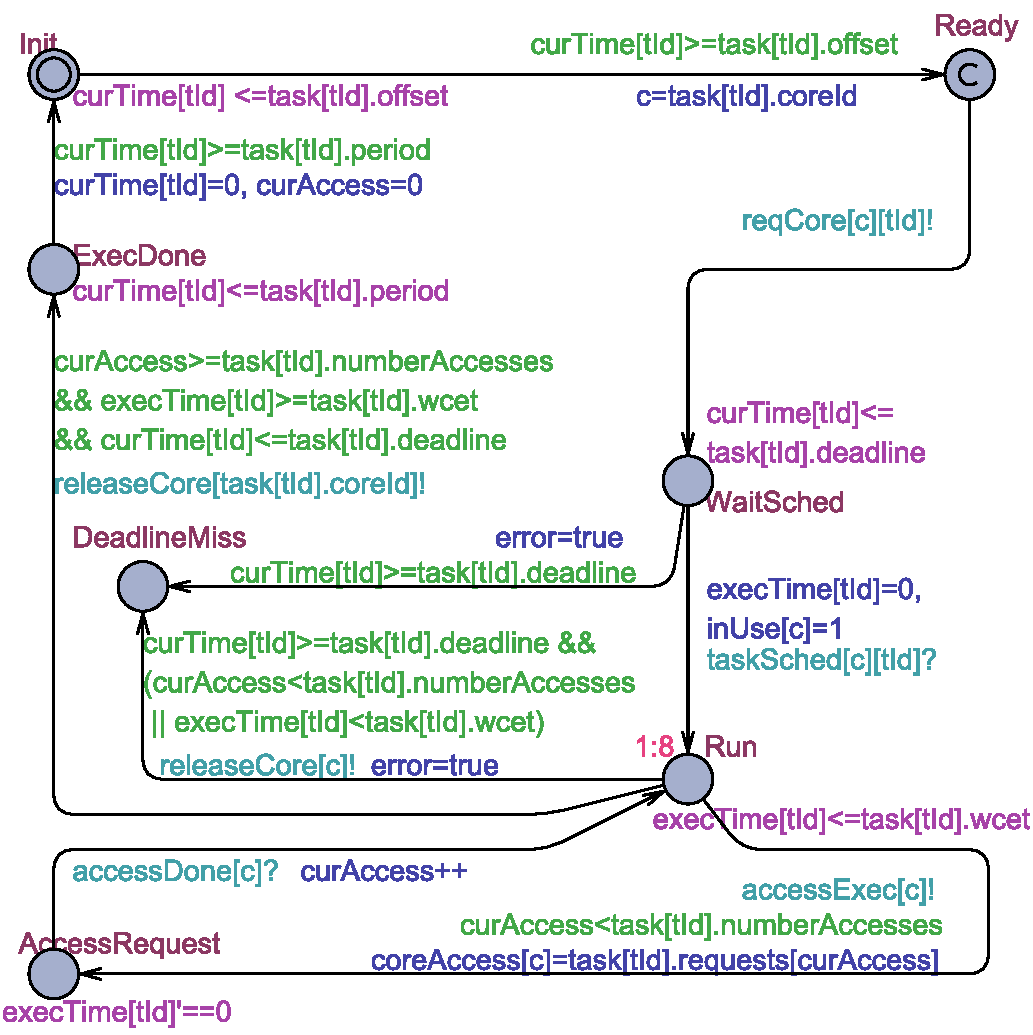
\includegraphics[scale=0.44]{Task.pdf}
\vspace{-7mm}
\end{figure}

Our Uppaal task template model is depicted in Fig.~\ref{fig:task}. To distinguish between different tasks, we associate to each task an identifier \texttt{tId} as a template parameter. The task starts at location \ft{Init} where it initializes its variables if needed, during the offset time. Once the offset expires, the task moves to location \ft{Ready} to request the core (\emph{c}) it is mapped to, through a synchronization with the core scheduler on channel \texttt{reqCore}. The task waits to be scheduled at location \ft{WaitSched} unless the deadline is reached by which it moves to location \ft{DeadlineMiss} and updates a global variable \emph{error} to true. Once a task is scheduled it updates the status of the corresponding core \emph{inUse[c]=1}, and moves to location \ft{Run} to execute. The status update of variable \emph{inUse[c]} leads the clock accumulating the core utilization to resume. During its execution (\emph{WCET}), a task non-deterministically triggers access requests to L2 and DRAM. For each access request, the task moves to location \ft{AccessRequest} and waits until the access request is satisfied upon which it moves back to location \ft{Run}. One can remark that, when a task is requesting and waiting for data the clock measuring \emph{WCET} is stopped (\emph{execTime[tId]'==0}) so that only the effective execution at \ft{Run} consumes \emph{WCET}. This is implemented in Uppaal by assigning rate 0 to the derivative of \emph{execTime[tId]}. Such a clock resumes at \ft{Run}. From \ft{Run}, the task joins either \ft{ExecDone}, if the execution \emph{WCET} and accesses to L2 and DRAM ($\emph{numberAccesses=WCRA}_c^r\emph{+WCRA}_c^w \emph{+WCRA}_m^r\emph{+WCRA}_m^w$) are completed before deadline, or it moves to location \ft{DeadlineMiss} in case the execution or access requests are not achieved before deadline. Once the period expires, at location \ft{ExecDone}, the task moves to \ft{Init} to start a new period. The task template can be instantiated for different tasks by just providing the aforementioned parameters.%, specified in the aforementioned definition.
  

\subsection{Platform Model}
A platform is given by a set of processing elements {\cal PE}, sharing a cache level L2 and DRAM memory, and schedulers to manage the access to L2 and DRAM. Each processing element PE is given by a computation resource (core), a local cache memory and a scheduler to dispatch tasks to run on that core. The access time for local caches may vary from one PE to another. In fact, such a number corresponds to a cache hit. In case of a cache miss, extra delay will result from accessing the shared memory. %Moreover, we consider the time duration for an effective access (from grant to completion) to a shared memory as a platform parameter. 

\subsubsection{Modeling of Processing Elements}
A processing element PE is given by $\langle C, sched, H\rangle$ where $C$ is a core, $sched$ is the scheduling policy (core scheduler) adopted and $H$ is the local cache that we abstract using its access time $LocalCacheTime$. The core model is depicted in Fig.~\ref{fig:core}.  

\begin{figure}
\centering
\caption{Core template model}
\label{fig:core}
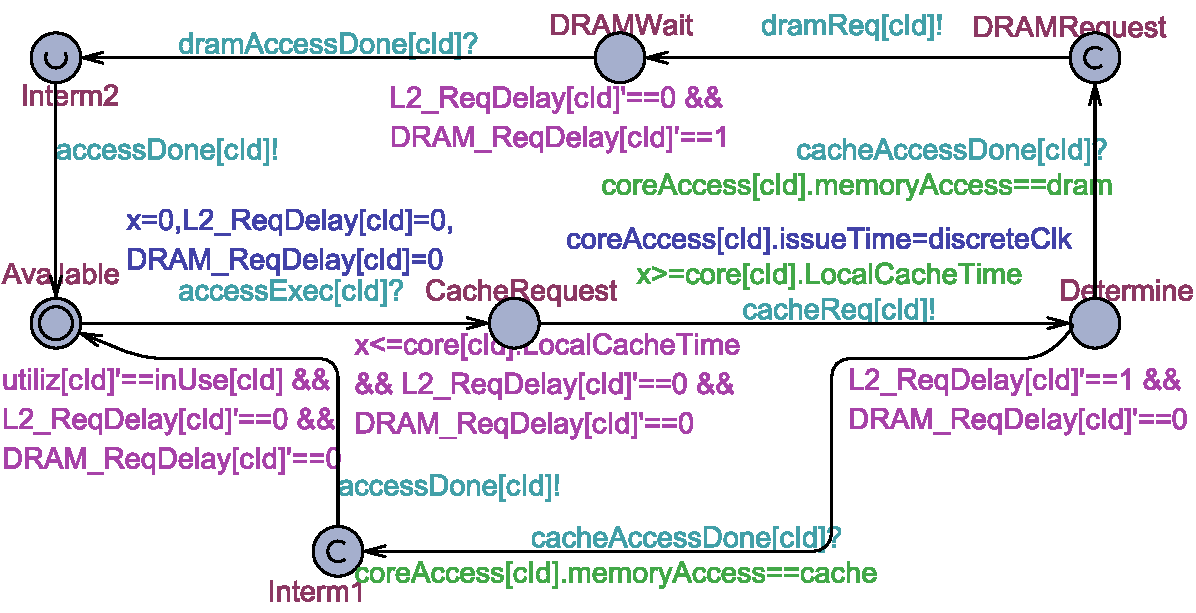
\includegraphics[scale=0.41]{Core.pdf}
\vspace{-3mm}
\end{figure}

Similarly to tasks, we assign to each core an identifier \texttt{cId} as a parameter to distinguish between the different platform cores. The core model is initially at location \ft{Available} waiting for ready tasks. Through an allocation, the core model does not move from \ft{Available} but the clock measuring its utilization \emph{utiliz[cId]} starts counting (\emph{utiliz[cId]'==inUse[cId]}). Such a clock can stop and resume according to the core status \emph{inUse[cId]} manipulated at task level. Upon an access request to a shared memory (\emph{accessExec[cId]?}), the core moves to location \ft{CacheRequest} where it waits for the expiry of the local cache access time \emph{LocalCacheTime} before performing the access request to the shared cache L2 and joins location \ft{Determine}. The core updates the request issue time with the current time instant \emph{issueTime=discreteClk}. At that location, the clock measuring the core delay for the current access to L2 starts (\emph{L2\_ReqDelay[cId]'==1}). 
Once the access to L2 hits (\emph{memoryAccess==cache}) and terminates, the clock \emph{L2\_ReqDelay[cId]} gets preempted (\emph{L2\_ReqDelay[cId]'==0}) and the core moves back immediately to location \ft{Available} to continue executing the assigned task. Otherwise, once the L2 access terminates and misses (\emph{memoryAccess==dram}) the core requests access to DRAM and joins immediately the location \ft{DRAMWait}, whereby the clock measuring the core delay for the current access request is released (\emph{DRAM\_ReqDelay[cId]'==1}). Once the current access is completed, clock \emph{DRAM\_ReqDelay[cId]} gets preempted while holding the measured delay. Upon the release of new access requests, from location \ft{Available}, clocks \emph{L2\_ReqDelay[cId]} and \emph{DRAM\_ReqDelay[cId]} are reset. 
  
The core blocking time on an access request (at locations \ft{Determine} and \ft{DRAMWait}) depends on the access nature. If it is a write action, the core will immediately be unlocked by the scheduler of the targeted memory, otherwise the core stalls until the read access finishes. Further details regarding how to handle read and write accesses will be provided in the description of L2 and DRAM schedulers.    

The core needs to notify the running task when the current access request is done, i.e. once the core itself is notified by DRAM or L2 (according to the access pattern), so that the task moves back as well from location \ft{AccessRequest} to \ft{Run} and accounts a granted access (\emph{curAccess++}). As it is not possible to entitle a transition with two synchronization events in Uppaal, we introduce two intermediate locations \ft{Interm1} and \ft{Interm2}. Thus, we create a sequence of 2 synchronizations without any delay between them. We use \textit{urgentness} and \textit{committedness} of Uppaal to enforce time to not elapse at a given location (locations marked with \texttt{U} and \texttt{C}).

\begin{figure}
\centering
\vspace{-2mm}
\caption{Scheduler template model}
\label{fig:sched}
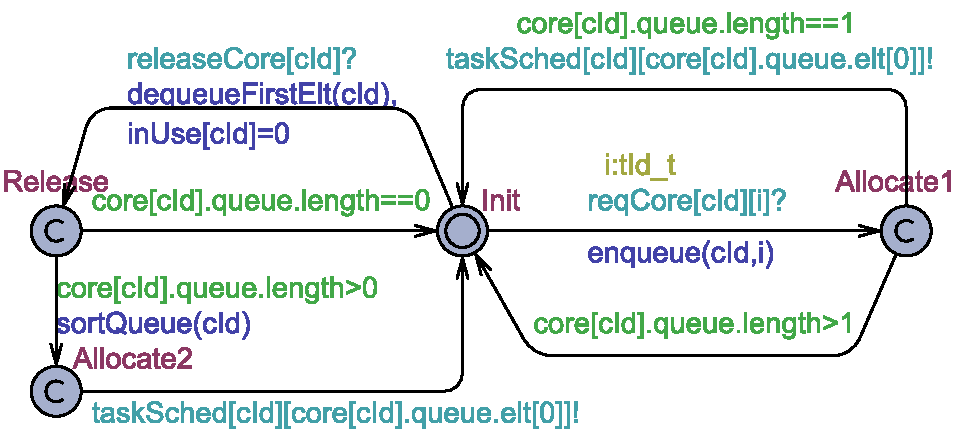
\includegraphics[scale=0.46]{Scheduler.pdf}
\vspace{-7mm}
\end{figure}

 Fig.~\ref{fig:sched} depicts the core scheduler model. Initially at location \ft{Init} waiting for a ready task request, the core moves to location \ft{Allocate1} while queuing the identifier of the requesting task. If the core queue contains only one element (\emph{queue.length==1}), which is the identifier of the newly added task, that task will immediately be scheduled otherwise the scheduler just moves back to \ft{Init}. Once the core is released by the current running task, through a signal on channel \emph{releaseCore}, the scheduler moves to \ft{Release} while removing the first element of the queue. If the queue is still not empty, the scheduler calls the adopted scheduling policy \emph{sortQueue()} of core $cId$ to sort the queue and moves to location \ft{Allocate2}, whereafter it schedules the task corresponding to the new first element in the queue. Function \emph{sortQueue(cId)} refers to the scheduling policy of core \emph{cId}, which is a core parameter in our model and can be FIFO, FPS, EDF or memory-centric.   
   
\subsubsection{Modeling of Shared Memories}
This section describes the modeling of L2 cache, DRAM and their schedulers.  
A DRAM=$\langle \emph{DRAMStruct, DRAMSched, DRAMAccessTime}\rangle$ is given by a structure \emph{DRAMStruct} (Fig.~\ref{fig:dram}), a scheduler \emph{DRAMSched} (Fig.~\ref{fig:dramsched}) and the time duration for an effective access \emph{DRAMAccessTime}. The DRAM access time simulates the duration of fetching data from a physical address in DRAM once the access is scheduled. This is in fact to enable our abstraction of the DRAM internal architecture to capture the delay for accessing a DRAM bank/row. Our DRAM model can be viewed as a one-bank memory that is shared between all cores, but it can easily be extended for several banks by just duplicating the DRAM structure and assigns each to one core only \cite{Heechul2015}. Moreover, we assume that the instantiation of our L2 and DRAM models satisfies the JEDEC standard \cite{Jedec}, which dictates the operation and timing constraints of memory devices such latency, opening and closing durations of banks.

%We omit specifying the size of DRAM neither the size of the cache space assigned to each application. The reason behind that is that the impact of these characteristics on the interference is already captured by $WCRA_m$ and $WCRA_c$, however the size of such spaces is a primordial element in the calculation of WCRAs and cache miss ratio.

The DRAM structure model (Fig.~\ref{fig:dram}) is initially waiting at location \ft{Idle} for an access request, either read or write. DRAM can be allocated, by its scheduler, to a given core \emph{i} performing a read request \emph{DRAMReqR[i]?} and moves to location \ft{Read}. Similarly, DRAM can be targeted with a write request \emph{DRAMReqW?}.

One can see that for write access requests the identifier of the involved core is missing. This is because write requests are not blocking, thus no need to keep track of which core needs to be unlocked once the access is done. At locations \ft{Read} and \ft{Write}, the DRAM waits for the expiry of the access time \emph{$DRAMAccessTime$} then moves to location \ft{Done}. From \ft{Read}, once the access time expires the DRAM unlocks the involved core through a synchronization \emph{dramAccessDone[currentCore]!}, whereas from location \ft{Write} no unlock action is needed. From \ft{Done}, DRAM notifies its scheduler that the current access is done, so that other requests can be performed.  
  
%Upon a read request, the DRAM is allocated to the requesting core and moves to location \ft{Access} where it waits for the effective access time $DRAMAccessTime$ to expire. Once such a duration expires, the DRAM notifies the requesting core so that it resumes its regular execution ($dramAccessDone!$). The DRAM notifies its scheduler as well that it becomes available to satisfy other potential requests ($releaseDRAM!$).   

\begin{figure}[ht]
\centering
\vspace{-3mm}
\caption{DRAM template model}
\label{fig:dram}
\vspace{-2mm}
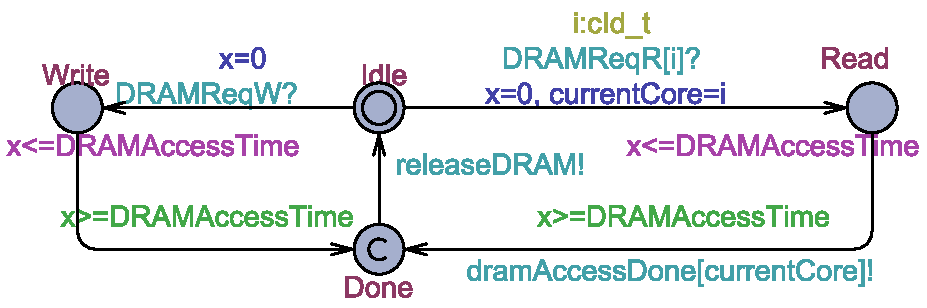
\includegraphics[scale=0.53]{DRAMMemory.pdf}
\vspace{-3mm}
\end{figure}

We adopt the FR-FCFS policy to arbitrate accesses to DRAM. We assume that row opening and reload actions are instantaneous, so that we do not need to consider any preference based on the \textit{already open row} policy \cite{Kim14}. This leads us to consider the attribute \emph{issueTime} of each request as a \textit{readiness}. Hence, we characterize each request to DRAM with another new attribute \emph{arrivalT}, besides to \emph{issueTime}. In fact, \emph{issueTime} stores the time instant when the request is issued, whereas \emph{arrivalT} stores the instant when the request reaches the corresponding bank queue. Thus, we compare requests first based on their issue times (readiness) where an earlier request has priority over later ones. If requests have the same issue time, then the request having an earlier \emph{arrivalT} has priority over requests having later \emph{arrivalT}. 

The DRAM scheduler is depicted in Fig.~\ref{fig:dramsched}. Initially at location \ft{Init}, upon the receive of an access request \emph{dramReq[i]?} from any core \emph{i} the DRAM scheduler inserts such a request together with the identifier of the requesting core into the queue and moves to location \ft{Allocate1}. If such a request is a write (\emph{rwAction==Write}), the requesting core will immediately be unlocked (\emph{dramAccessDone[l]!}) as location is committed \ft{Allocate1}. Moreover, the write request is alone in the queue (\emph{queue.length==1}) it will immediately be scheduled at location \ft{Unlocked}.
In case of a read request (\emph{rwAction==Read}), the DRAM scheduler does not unlock the requesting core after queuing the request, but it just schedules the access (\emph{DRAMReqR[DRAM.queue.elt[0].core]!}) if the current request is alone in the queue. In all of the four scenarios, the scheduler moves back to location \ft{Init}.

Once an access request is performed, the scheduler is notified by the DRAM through a synchronization event \emph{releaseDRAM?} and moves to \ft{Release} while removing the head of the queue. If the queue is still not empty, the scheduler calls the algorithm FR-FCFS to sort the queue as other requests might join during the execution of the last access. At location \ft{Allocate2}, the scheduler schedules the request in the first element of the queue \emph{queue.elt[0]} using the appropriate channel (\emph{DRAMReqR} or \emph{DRAMReqW}) according to the request nature; read or write.  

\begin{figure}[htb]
\centering
\vspace{-3mm}
\caption{DRAM scheduler model}
\label{fig:dramsched}
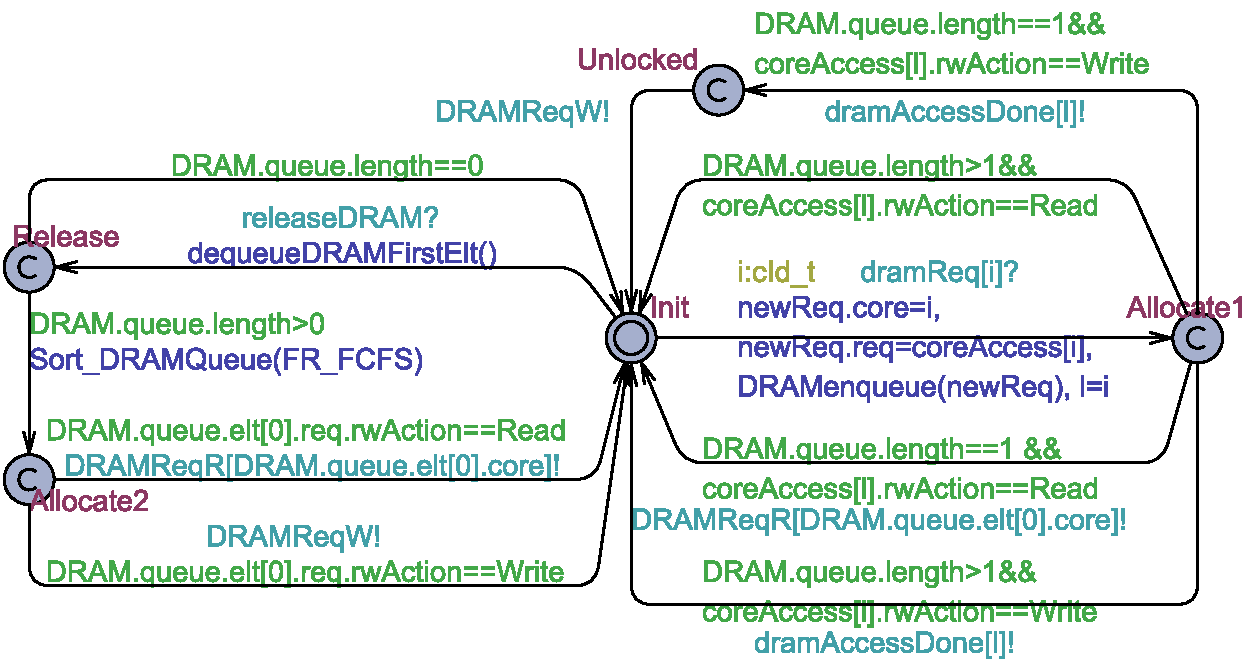
\includegraphics[scale=0.41]{DRAMScheduler.pdf}
\vspace{-3mm}
\end{figure}

Due to space limitations, we omit describing the shared cache L2 and its scheduler. In essence, L2 has the same elements as DRAM , except that it uses a separate queue to store its requests. Similarly, L2 scheduler has the same behavior as that of DRAM but it operates on the L2 queue using the cache coloring policy. However, since we do not consider the internal pages of L2, the coloring policy adopted in our framework behaves in similar way to FCFS policy.

Finally, a platform \emph{P} is given by \begin{footnotesize}\emph{$\langle \langle PE_1, .., PE_m \rangle, DRAM, L2\rangle$}\end{footnotesize}. One can see that updating the specification of one platform ingredient does not necessarily affect the others. %In case a new memory connector needs to be used instead (for example FCFS), we simply replace the bus $B$ with the new connector. 

\subsection{System Model}
In order to make our framework flexible, the application and platform are specified separately then mapped together. A system model $S$ is given by an application \emph{$AP=\{T_1,..,T_n\}$}, a platform \emph{$P=\langle {\cal PE}, DRAM, L2\rangle$} and a mapping \emph{$M:AP \rightarrow {\cal PE}$} assigning each task to a processing element \emph{$PE_i \in {\cal PE}$}. %A task can only be assigned to one core, however a core can serve different tasks.

